%
% loesung.tex -- Beispiel-File für die Beschreibung der Loesung
%
% (c) 2020 Prof Dr Andreas Müller, Hochschule Rapperswil
%
\section{Lösung
\label{quadratur:section:loesung}}
\rhead{Lösung}
\subsection{Anwendung der Gauss-Legendre-Formel
\label{quadratur:subsection:gausslegendreanwendung}}
In dieser Subsektion versuchen wir, die Verwendung der Gauss-Legendre-Formel in einem
einfachen Beispiel herzuleiten, hierzu wird wieder die Funktion  
$I = \int_{-1}^{1}\sqrt{(1-x^2)}\,dx$ verwendet und 
wir berechnen die Formel mit vier Stützstellen.
\newline

Zudem werden in der Tabelle~\ref{buch:table:gaussbeispielwerte} die Werte der 
Stützstellen und der Gewichte angegeben. Die Berechnung der Stützstellen, der Gewichte
und die verschiedenen Formen der Gauss-Quadratur werden in den folgenden Sektionen 
hergeleitet.

\begin{table}[h!]
    \centering
    \begin{tabular}{|c|c|}
        \hline
        Stützstellen $x_{i}$ & Gewichte $A_{i}$ \\
        \hline
        $-0.861136 $ & $ 0.347855 $ \\
        $-0.339981 $ & $ 0.652145 $ \\
        $\phantom{-} 0.339981 $ & $ 0.652145 $ \\
        $\phantom{-} 0.861136 $ & $ 0.347855 $ \\
        \hline
    \end{tabular}
    \caption{Werte für vier Stützstellen und deren Gewichte
    \label{buch:table:gaussbeispielwerte}}    
\end{table}

\noindent
In der Abbildung~\ref{quadratur:figure:gausslegendre1} sind die vier Stützstellen 
ersichtlich.

\begin{figure}[!h]
    \centering
    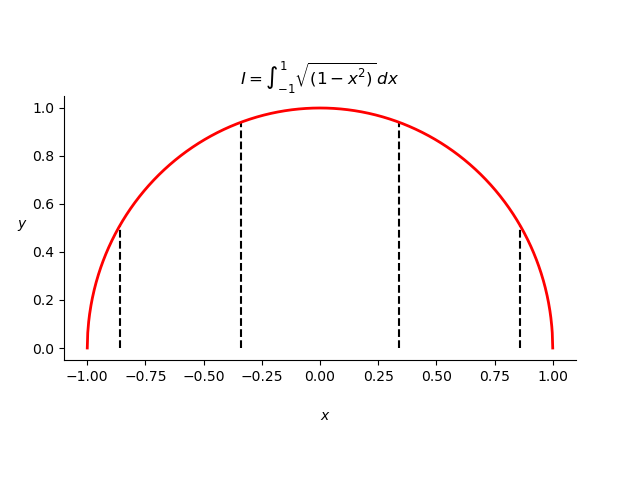
\includegraphics[scale=0.7]{papers/quadratur/figures/GaussLegendre1.png}
    \caption{ Position der Stützstellen
    \label{quadratur:figure:gausslegendre1}}
\end{figure}

\newpage
\noindent
Die Fläche unter dem Integral lässt sich nun mit der Formel 

\begin{equation}
    I 
    =
    \int_{-1}^{1} f(x) 
    \approx
    \sum_{i=0}^{n} A_{i} f(x_{i})
\end{equation}
\noindent 
berechnen, indem man die Stützstellen $x_{i}$ und die Gewichte $A_{i}$ einsetzt.

    \begin{align}
        I 
        &\approx 
        0.347855 \cdot \sqrt{1-(-0.861136)^{2}} 
        \notag
        \\
        &+ 
        0.652145 \cdot \sqrt{1-(-0.339981)^{2}} 
        \notag
        \\
        &+ 
        0.652145 \cdot \sqrt{1-(0.339981)^{2}} 
        \notag
        \\
        &+ 
        0.347855 \cdot \sqrt{1-(0.861136)^{2}} 
        \notag
        \\
        \notag
        \\
        &\approx 2 \cdot 0.652145 \cdot \sqrt{1-(0.339981)^{2}} + 2 \cdot 0.347855 \cdot \sqrt{1-(0.861136)^{2}} 
        \notag
        \\
        &\approx 1.226596 + 0.386863 
        \notag
        \\
        &\approx 1.580278
    \end{align}

\noindent
Das Resultat $1.580278$ ist bereits deutlich besser an der tatsächlichen Fläche $1.570796$ 
angenähert, als die Resultate der Trapezformel. 

\subsection{Berechnung der Position der Stützstellen
\label{quadratur:subsection:stützstellenberechnung}}
Um die Position der Stützstellen zu bestimmen, benötigt man zuerst die Anzahl Stützstellen, 
die für die Quadratur einer Funktion benötig werden.
\noindent
Wie im Abschnitt~\ref{quadratur:section:problemstellung} erwähnt, 
kann man mit $n$ Stützstellen das Integral eines Polynoms vom Grad $2n-1$ exakt berechnen.
Anders ausgedrückt: Hat man ein Polynom vom Grad $g$, 
benötigt man für eine exatkte Berechnung des Integrals $\frac{g+1}{2}$ Stützstellen.
Hat man eine Funktion, die sich nicht als Polynom darstellen lässt, 
kann man die Funktion durch ein Polynom annähern, 
oder die Anzahl benötigter Stützstellen schätzen.
Falls man die Anzahl Stützstellen schätzt, ist darauf zu achten, 
dass eine grössere Anzahl zwar die Genauigkeit der Quadratur erhöht,
aber auch der Berechnungsaufwand grösser wird.


\subsubsection{Beispiel: Polynom vom Grad $7$}
Angenommen, man hat die Funktion $f(x) = 5 \cdot x^{7} + 2 \cdot x^{5} - 8 \cdot x^{3} + x + 3$.
Der Grad der Funktion lässt sich aus dem höchsten vorkommenden Exponenten von $x$ ableiten,
also $7$.
Für ein Polynom vom Grad $7$ werden $\frac{7+1}{2} = 4$ Stützstellen benötigt.
In der Abbildung~\ref{quadratur:figure:polynom} ist die Funktion mit den vier 
Stützstellen ersichtlich.

\begin{figure}[!h]
    \centering
    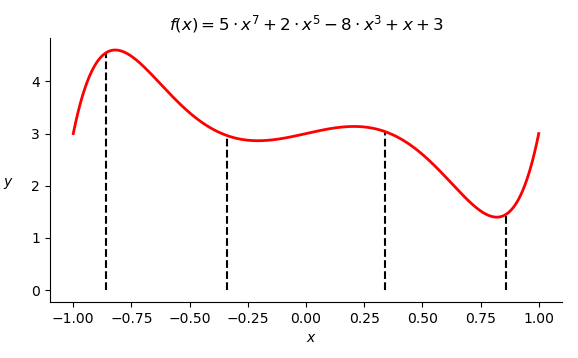
\includegraphics[scale=0.7]{papers/quadratur/figures/polynom.png}
    \caption{ Funktion des Polynom mit vier Stützstellen
    \label{quadratur:figure:polynom}}
\end{figure}
\newpage
\noindent
Mit dem selben Beispiel lässt sich auch erklären, warum für ein Polynom vom Grad $n$ 
weniger als $n$ Stützstellen benötigt werden.
\noindent
Berechnet man das Integral eines ungeraden Terms
\begin{equation}
    \int_{-1}^{1}x^{2k-1}\,dx 
    =
     \frac{1}{2k} \cdot x^{2k} \bigg|_{-1}^{\phantom{-}1}
    = 
    0
\end{equation} 
sieht man, dass ungerade Koeffizienten verschwinden. 
Für die Berechnung der Anzahl Stützstellen werden somit 
nur die Anzahl der geraden Koeffizienten benötigt.
\newline
\subsubsection{Beweis}
\begin{equation}
    \int_{-1}^{1}x^{2}
    =
    \frac{x^{3}}{3} \bigg|_{-1}^{1}
    = 
    \bigg(\frac{1^{3}}{3}\bigg) - \bigg(\frac{(-1)^{3}}{3}\bigg)
    = 
    \frac{1}{3} - \frac{-1}{3}
    =
    \frac{2}{3}
\end{equation}
\begin{equation}
    \int_{-1}^{1}x^{3}
    =
    \frac{x^{4}}{4} \bigg|_{-1}^{1}
    = 
    \bigg(\frac{1^{4}}{4}\bigg) - \bigg(\frac{(-1)^{4}}{4}\bigg)
    = 
    \frac{1}{4} - \frac{1}{4}
    =
    0
\end{equation}
\begin{equation}
    \int_{-1}^{1}x^{4}
    =
    \frac{x^{5}}{5} \bigg|_{-1}^{1}
    = 
    \bigg(\frac{1^{5}}{5}\bigg) - \bigg(\frac{(-1)^{5}}{5}\bigg)
    = 
    \frac{1}{5} - \frac{-1}{5}
    =
    \frac{2}{5}
\end{equation}
\begin{equation}
    \int_{-1}^{1}x^{5}
    =
    \frac{x^{6}}{6} \bigg|_{-1}^{1}
    = 
    \bigg(\frac{1^{6}}{6}\bigg) - \bigg(\frac{(-1)^{6}}{6}\bigg)
    = 
    \frac{1}{6} - \frac{1}{6}
    =
    0
\end{equation}
\newline
\noindent
Weiss man, wieviele Stützstellen $n$ man für die Berechnung der Quadratur verwenden möchte,
kann man die Position der Stützstellen berechnen. 
Dafür hat man zwei Möglichkeiten, welche nachfolgend erklärt werden.

\newpage

\subsubsection{Werte in der Tabelle nachschlagen}
Für die gängigsten Formen der Gauss-Quadratur existieren Tabellen mit vorberechneten Werten für die
Position der Stützstellen und deren Gewichte. 
Es ist möglich, dass für grosse $n$ keine Tabellenwerte gefunden werden und die Berechnung 
selber durchgeführt werden muss.

In der Tabelle~\ref{buch:table:gaussabscissenwerte} sind die Werte für $n \leq 6$ beschrieben.

\begin{table}[h!]
    \centering
    \begin{tabular}{|c|c|}
        \hline
        $n$ & Stützstellen $x_{i}$ für $n$ \\
        \hline
        $1$ & $ \phantom{-} 0.00000 $ \\
        \hline
        $2$ & $ \pm 0.57735 $ \\
        \hline
        $3$ & $ \pm 0.77460 $ \\
            & $ \phantom{-} 0.00000 $ \\
        \hline
        $4$ & $ \pm 0.86114 $ \\
            & $ \pm 0.33998 $ \\
        \hline
        $5$ & $ \pm 0.90618 $ \\
            & $ \pm 0.53847 $ \\
            & $ \phantom{-} 0.00000 $ \\
        \hline
        $6$ & $ \pm 0.93247 $ \\
            & $ \pm 0.66121 $ \\
            & $ \pm 0.23862 $ \\
        \hline
    \end{tabular}
    \caption{Werte für Stützstellen $x_{i}$ der Gaussquadratur für $n \leq 6$
    \label{buch:table:gaussabscissenwerte}}    
\end{table}

\subsubsection{Berechnen durch Formel}
Die Position der Stützstellen lässt sich mit der Formel

\begin{equation*}
    \int_{-1}^{1} P(x) \cdot x^{j} \, dx = 0
\end{equation*}

\noindent
mit

\begin{equation*}
    j = 0, 1, 2, ... n - 1
\end{equation*}

\noindent
und 

\begin{equation}
    P(x) = (x - x_{1})(x - x_{2}) ... (x - x_{n})
\end{equation}
\noindent
berechnen.
\newline

\noindent
Um die Formel zu verstehen, werden einige Grundkenntnisse für 
orthogonale Polynome und deren beziehung zur Gauss-Quadratur vorausgesetzt.
Da aber für die häufigsten Formen der Gauss-Quadratur 
(Siehe Abschnitt ~\ref{quadratur:subsection:gaussformen}) bereits vorberechnete
Tabellen für die Stützstellen und Gewichte existieren muss man die Theorie
für die Anwendung der Formeln nicht verstehen. Für interessierte Leser sind 
die wichtigsten Eigenschaften von orthogonalen Polynomen im nächsten 
Abschnitt genäuer erläutert.
\newpage

\subsubsection{Orthogonale Polynome}
Orthogonale Polynome werden in der mathematischen und 
numerischen Analysis oft verwendet.
In der numerischen Integration werden Eigenschaften dieser Polynome für
die Berechnung der Stützstellen und Gewichte benötigt.
\newline

\noindent
Zwei Polynome $\phi_{m}(x)$ und $\phi_{n}(x)$ 
($n$ und $m$ ist hierbei der Grad des Polynoms) formen ein 
orthogonales Paar im intervall $(a, b)$ im Bezug auf die Gewichtungsfunktion
$w(x)$ falls:
\begin{equation}
    \int_{a}^{b} w(x) \phi_{m}(x) \phi_{n}(x)\,dx = 0 \, , m \neq n
\end{equation}

\noindent
Orthogonalpolynome sind abgesehen vom konstanten Faktor, über die Wahl der
Gewichtungsfunktion und der Grenzen des Integrals $a, b$, festgelegt.
Klassische Orthogonalpolynome sind nach bekannten Mathematikern 
benannt und in der Tabelle~\ref{buch:table:orthogonalpolynomials} mit ihren
Eigenschaften beschrieben.

\begin{table}[h!]
    \centering
    \begin{tabular}{|c|>{$}c<{$}|>{$}c<{$}|>{$}c<{$}|>{$}c<{$}|}
        \hline
        Name & \text{Symbol} & a & b & w(x) \\
        \hline
        Legendre & p_{n(x)} & -1 & 1 & 1 \\
        Chebyshev & T_{n}(x) & -1 & 1 & (1-x^{2})^-1/2 \\
        Laguerre & L_{n}(x) & \phantom{-}0 & \infty & e^{-x} \\
        Hermite & H_{n}(x) & -\infty & \infty & e^{-x^{2}} \\
        \hline
    \end{tabular}
    \caption{Klassische Orthogonalpolynome
    \label{buch:table:orthogonalpolynomials}}    
\end{table}


\noindent
Weiterhin haben Orthogonale Polynome rekursive Beziehungen zueinander, das heisst,
dass mit der Formel
\begin{equation}
    a_{n}\phi_{n+1}(x) = (b_{n} + c_{n}x)\phi_{n}(x) - d_{n}\phi_{n-1}(x)
\end{equation}

\noindent
mit den ersten beiden Orthogonalpolynomen die restliche Menge der Polynome berechnet werden kann,
die zueinander orthogonal sind. Die Koeffizienten für die Formel finden sich in der 
Tabelle~\ref{buch:table:orthogonalcoefficients}

\begin{table}[h!]
    \centering
    \begin{tabular}{|c|>{$}c<{$}|>{$}c<{$}|>{$}c<{$}|>{$}c<{$}|>{$}c<{$}|>{$}c<{$}|}
        \hline
        Name & \phi_{0}(x) & \phi_{1}(x) & a_{n} & b_{n} & c_{n} & d_{n} \\
        \hline
        Legendre & 1 & x & n + 1 & 0 & 2n + 1 & n \\
        Chebyshev & 1 & x & 1 & 0 & 2 & 1 \\
        Laguerre & 1 & 1 - x & n + 1 & 2n + 1 & -1 & n \\
        Hermite & 1 & 2x & 1 & 0 & 2 & 2 \\
        \hline
    \end{tabular}
    \caption{Koeffizienten für die berechnung von Orthogonalpolynomen
    \label{buch:table:orthogonalcoefficients}}    
\end{table}

Weitere für die Gaussquadratur relevante Eigenschaften von Orthogonalpolynomen:
\begin{itemize}
    \item Ein Polynom $\phi_{n}(x)$ vom Grad $n$ hat $n$ reelle, unterschiedliche Nullstellen im Intervall $(a, b)$.
    \item Nullstellen des Polynoms $\phi_{n}(x)$ liegen zwischen den Nullstellen des Polynoms $\phi_{n+1}(x)$.
    \item Ein beliebiges Polynom $P_{n}(x)$ kann in der Form 
    $P_{n}(x) = \sum_{i=0}^{n} c_{i}\phi_{i}(x)$
    ausgedrückt werden
    \item Daraus, und aus den Orthogonalitätseigenschaften folgt die folgende Formel:
    \begin{equation}
        \int_{a}^{b} w(x) P_{n}(x)\phi_{n+m}(x)\, dx = 0, \, m\ge0 
    \end{equation}
\end{itemize}
\newpage

\subsubsection{Beispiel: Berechnung für zwei Stützstellen}
Möchte man die Position für zwei Stützstellen berechnen, sieht die Formel folgendermassen aus:

\begin{equation}
    P(x) = (x - x_{1})(x - x_{2})
\end{equation}

\noindent
und man erhält für $j = 0,1$ die beiden Gleichungen

\begin{equation*}
    \int_{-1}^{1}(x - x_{1})(x - x_{2}) \; dx = 0
\end{equation*}

\begin{equation*}
    \int_{-1}^{1}(x - x_{1})(x - x_{2})x \; dx = 0
\end{equation*}

\noindent
Löst man das Integral, erhält man:

\begin{equation*}
    \frac{1}{3} + x_{1}x_{2} = 0
\end{equation*}

\begin{equation}
    \frac{2}{3}(x_{1}+x_{2}) = 0
\end{equation}

\noindent
Umgeformt erhält man:

\begin{equation}
    x_{1}x_{2} = -\frac{1}{3}
    \;
    \text{und}
    \;
    x_{1}+x_{2} = 0
\end{equation}

\noindent
Somit sind $ x_{1} $ und $ x_{2} $:

\begin{equation*}
    x_{1} = -\frac{1}{\sqrt{3}} \approx -0.55735
\end{equation*}

\begin{equation}
    x_{2} = \phantom{-} \frac{1}{\sqrt{3}} \approx \phantom{-}0.55735
\end{equation}

\newpage

\subsection{Berechnung der Gewichte an den Stützstellen
\label{quadratur:subsection:gewichtsberechnung}}
Auch für die Bestimmung der Gewichte an den berechneten Stützstellen kann man entweder
in einer vorberechneten Tabelle die Werte nachschlagen, oder die Gewichte selber berechnen.

\subsubsection{Tabelle für die Gewichte}
In der Tabelle~\ref{buch:table:gaussgewichtwerte} sind für $ n \leq 6 $ die Gewichte $A_{i}$
an den Stützstellen $x_{i} $ angegeben.

\begin{table}[h!]
    \centering
    \begin{tabular}{|c|c|c|}
        \hline
        $n$ & Stützstellen $x_{i}$ für $n$ & Gewichte $A_{i}$\\
        \hline
        $1$ & $ \phantom{-} 0.00000 $ & $ 2.00000 $ \\
        \hline
        $2$ & $ \pm 0.57735 $ & $ 1.00000 $ \\
        \hline
        $3$ & $ \pm 0.77460 $ & $ 0.55556 $ \\
            & $ \phantom{-} 0.00000 $ & $ 0.88889 $ \\
        \hline
        $4$ & $ \pm 0.86114 $ & $ 0.34785 $ \\
            & $ \pm 0.33998 $ & $ 0.65215 $ \\
        \hline
        $5$ & $ \pm 0.90618 $ & $ 0.23693 $ \\
            & $ \pm 0.53847 $ & $ 0.47863 $ \\
            & $ \phantom{-} 0.00000 $ & $ 0.56889 $ \\
        \hline
        $6$ & $ \pm 0.93247 $ & $ 0.17132 $ \\
            & $ \pm 0.66121 $ & $ 0.36076 $ \\
            & $ \pm 0.23862 $ & $ 0.46791 $ \\
        \hline
    \end{tabular}
    \caption{Werte für Stützstellen $x_{i}$ und Gewichte $A_{i}$ der Gaussquadratur für $n \leq 6$
    \label{buch:table:gaussgewichtwerte}}    
\end{table}

\subsubsection{Berechnen der Gewichte}
Die Gewichte an den Stützstellen lässt sich mit der Formel

\begin{equation*}
    A_{j} = \int_{-1}^{1} l_j(x) \, dx
\end{equation*}

\noindent
mit

\begin{equation*}
    j = 1, 2, ... , n
\end{equation*}

\noindent
und 

\begin{equation}
    l_{j}(x) := \prod_{0 \leq m \leq k, \, m \neq j} \frac{x - x_{m}}{x_{j} - x_{m}}
\end{equation}

\noindent
berechnen.

\newpage

\subsubsection{Beispiel: Berechnung der Gewichte für zwei Stützstellen}
In der Beispielberechnung der Stützstellen in der 
Sektion~\ref{quadratur:subsection:stützstellenberechnung} sieht man, dass sich die 
Stützstellen an den Punkten $x_{1} = -\frac{1}{\sqrt{3}} $ und $x_{2} = \frac{1}{\sqrt{3}} $ befinden.

\noindent
Die Formeln für die Berechnung der Gewichte $A_{1}$ und $A_{2}$ sind:

\begin{equation*}
    A_{1} = \int_{-1}^{1} \frac{x - x_{2}}{x_{1} - x_{2}} \, dx
\end{equation*}

\noindent
und

\begin{equation}
    A_{2} = \int_{-1}^{1} \frac{x - x_{1}}{x_{2} - x_{1}} \, dx
\end{equation}


\noindent
setzt man die Werte für $x_{1}$ und $x_{2}$ in die Formeln ein, erhält man:

\begin{equation*}
    A_{1} = \int_{-1}^{1} \frac{x - \frac{1}{\sqrt{3}}}{\frac{-1}{\sqrt{3}} - \frac{1}{\sqrt{3}}} \, dx
\end{equation*}

\begin{equation}
    A_{2} = \int_{-1}^{1} \frac{x - \frac{-1}{\sqrt{3}}}{\frac{1}{\sqrt{3}} - \frac{-1}{\sqrt{3}}} \, dx
\end{equation}

\noindent
vereinfacht man die Terme, erhält man:

\begin{equation*}
    A_{1} 
    =
    \int_{-1}^{1} -\frac{1}{2} 
    \cdot \sqrt{3} 
    \cdot \bigg(x - \frac{1}{\sqrt{3}}\bigg)
    \, dx
    =
    -\frac{\sqrt{3}}{2} 
    \bigg(
    \cdot \int_{-1}^{1}x\,dx
    -
    \frac{1}{\sqrt{3}} 
    \cdot \int_{-1}^{1}1\,dx
    \bigg)
\end{equation*}

\begin{equation}
    A_{2} 
    =
    \int_{-1}^{1} \frac{1}{2} 
    \cdot \sqrt{3}  
    \cdot \bigg(x + \frac{1}{\sqrt{3}}\bigg)
    \, dx
    =
    \frac{\sqrt{3}}{2} 
    \bigg(
    \cdot \int_{-1}^{1}x\,dx
    +
    \frac{1}{\sqrt{3}} 
    \cdot \int_{-1}^{1}1\,dx
    \bigg)
\end{equation}

\noindent
$\int_{-1}^{1}x\,dx$ ist $0$ und $\int_{-1}^{1}1\,dx$ ist $2$, somit:

\begin{equation*}
    A_{1} 
    =
    -\frac{\sqrt{3}}{2} 
    \cdot 
    \bigg( 0
    -
    \frac{1}{\sqrt{3}} 
    \cdot 2
    \bigg)
    =
    1
\end{equation*}

\begin{equation}
    A_{2} 
    =
    \frac{\sqrt{3}}{2} 
    \cdot
    \bigg( 0
    +
    \frac{1}{\sqrt{3}} 
    \cdot 2
    \bigg)
    = 
    1
\end{equation}

\newpage


\subsection{Formen der Gauss-Quadratur
\label{quadratur:subsection:gaussformen}}
Wie im Abschnitt~\ref{quadratur:subsection:stützstellenberechnung}, 
Orthogonale Polynome bereits angedeutet, 
gibt es verschiedene Ausprägungen der Gauss-Integration.
Für verschiedene Folgen von Orthogonalpolynomen gibt es eine dazugehörige
Form der Gaussquadratur mit eigenen Grenzwerten und Berechnungsformeln.
Die vier häufigsten Formen sind in der Tabelle~\ref{buch:table:gaussformen} abgebildet.

\begin{table}[h!]
    \begin{tabular}{|>{$}c<{$}|>{$}c<{$}|>{$}c<{$}|>{$}c<{$}|}
        \hline
        \text{Name} &  \text{Untere Grenze} & \text{Obere Grenze} & \text{Formel} \\
        \hline  
        \text{Legendre} & -1 & 1 & p_{n}(x) = \int_{-1}^{1} f(x)\,dx \approx \sum_{i=0}^{n} A_{i} f(x_{i}) \\
        \text{Chebyshev} &  -1 & 1 & T_{n}(x) = \int_{-1}^{1} (1-x^{2})^{-1/2} f(x)\,dy \approx \frac{\pi}{n+1} \sum_{i=0}^{n} f(x_{i}) \\
        \text{Laguerre} &  0 & \infty & L_{n}(x) = \int_{0}^{\infty} e^{-x} f(x)\,dx \approx \sum_{i=0}^{n} A_{i} f(x_{i}) \\
        \text{Hermite} & -\infty & \infty & H_{n}(x) = \int_{-\infty}^{\infty} f(x)\,dx \approx \sum_{i=0}^{n} A_{i} f(x_{i})\\
        \hline
    \end{tabular}
    \caption{Formen der Gauss-Quadratur
    \label{buch:table:gaussformen}}   
\end{table}

\noindent
In den bisherigen Beispielen wurde die Gauss-Legendre Formel verwendet.
Interessant ist bei der Gauss-Chebyshev Formel, 
dass für die Berechnung des Integrals keine Gewichte berechnet werden müssen,
sondern dass für jedes $x_{i}$ das selbe Gewicht $\frac{\pi}{n+1}$ verwendet werden kann.

\noindent
Möchte man nun ein beliebiges Integral mittels der Gaussquadratur berechnen,
deren Grenzwerte nicht zu den in der Tabelle~\ref{buch:table:gaussformen} 
dargestellten Formeln passt, 
abgesehen von weiteren hier nicht genannten Formen, 
muss man die Grenzwerte $(a, b)$ gemäss dem Folgenden Beispiel
auf den Bereich $(-1, 1)$ abbilden.


\noindent
Angenommen man hat ein Integral
\begin{equation}
    \int_{a}^{b}f(x)\,dx
\end{equation}

\noindent
Mit der Transformation
\begin{equation}
    x = \frac{b + a}{2} + \frac{b - a}{2}\xi    
\end{equation}

\noindent
wird $dx = d\xi(b - a)/2$, und die Quadraturformel wird
\begin{equation}
    \int_{a}^{b}f(x)\,dx = \frac{b - a}{2} \int_{-1}^{1}f(\frac{b - a}{2}\xi + \frac{b + a}{2})\, d\xi \approx \frac{b - a}{2} \sum_{i=1}^{n} A_{i}f(x_{i})
\end{equation}
    
\newpage

\subsection{Fehler der Gauss-Quadratur
\label{quadratur:subsection:gaussfehler}}



\textcolor{red}{
    TODO
    \begin{itemize}
        \item Gauss Legendre Formel zeigen (Done)
        \item Beispiel berechnen mit Formel (Done)
        \item Berechnung der Position der Stützstellen (Done)
        \item Berechnung der Gewichtung (Done)
        \item Erklären der verschiedenen Formen der Gauss-Quadratur und ihrer Anwendungen (Done)
        \item Fehler der Gauss-Quadratur
    \end{itemize}
}
